
\section{Natural Phenomena as Metaphors for Software Maps}
\label{sec:metaphors}
\noindent
The proposed concept of trend maps is a metaphorical extension to existing interactive software maps. 
However, there are various definitions of metaphors in multiple science disciplines. 
Hereinafter, a metaphor consists of a \emph{target domain}, \emph{target item}, \emph{source domain}, \emph{source item}, and \emph{matching part} \cite{Zhang2008}.
The source item (\eg weathering effect) from a well-known source domain (natural phenomena) is mapped to target items (cuboids representing software entities) of the target domain (software maps).
The target domain is relatively unknown and the match will never be perfect.
However, the larger the matching part the better the metaphor works.

\begin{figure*}[t]
	\centering
	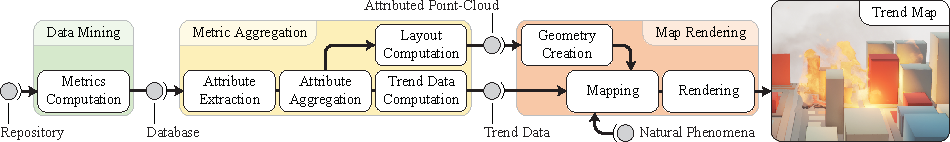
\includegraphics[width=1.0\textwidth]{pipeline}
	\caption{Schematic overview (data and control flow) of our trend map pipeline comprising three conceptual stages.}
	\label{fig:pipeline}
\end{figure*}

\subsection{Preliminaries and Assumptions}
\noindent
For the usage of natural phenomena we assume an appropriate match. 
This assumption is made due to our prior experience in assessing the semantics of natural phenomena. 
Furthermore, it is based on human usage of linguistic metaphors in idioms concerning natural phenomena such as \enquote{to go up in flames} and \enquote{grow grass upon}.
\Wrt the application and design of natural phenomena, we further assume that their image-synthesis can be performed in real-time to facilitate an interactive system.
Therefore, this paper focuses on hardware-accelerated rasterization for real-time rendering \cite{Akenine2008}.

\subsection{Conceptual Overview}
\noindent
Our approach is structured as pipeline comprising data mining, metrics aggregation, and trend map rendering (\autoref{fig:pipeline}).

\paragraph*{Data Mining}
\noindent
At first, software metrics are computed on a per-item basis. 
Therefore, each revision of a software system is analyzed independently.
The resulting artifact is a \emph{database} encoding a revision tree per revision.
This step is performed once for a given repository and allows for successive updates if new revisions have to be considered.

\paragraph*{Metric Aggregation}
\noindent
In this stage, a revision range $R = [n,\;m]$ with $n,m \in \mathbb{N}, n < m$ is specified by the user and used to compute the trend data later.
The user also selects the metrics of which he wants to observe trends.
The trend data of every treemap item is defined as a time series of metric data points over the revision range: 
For example, items that already existed at the start revision $n$ and outlast the end revision $m$, consist of a time series with $m-n+1$ data points.
Trend data is then aggregated with respect to particular parent items of the hierarchy. 
Subsequently, a treemap layout is computed and encoded as \emph{attributed point-cloud} for efficient rendering in the next stage. 
Simultaneously, the \emph{trend data} is computed by analyzing the time series for all treemap items.

\paragraph*{Map Rendering}
\noindent
The rectangular treemap geometry is created based on the attributed point cloud. 
Trends are mapped to the parametrization of natural phenomena (\autoref{sec:design_and_parametrization}).
Depending on the degree of change, five discrete levels are depicted in one trend map to facilitate visual distinction: strong increase, moderate increase, stagnation, moderate decrease, and strong decrease.
Up to two distinct effects can be specified by the user, one for negative and one for a positive trend. 
The effects are parametrized according to the computed trend and combined with the static system structure encoded in the attributed point-cloud.
The latter is used for final image synthesis (\autoref{sec:implementation}).

\section{Design and Parametrization of Natural Phenomena}
\label{sec:design_and_parametrization}
\noindent
Before focusing on suitable metaphors and their automatic parametrization, this section describes the design space of natural phenomena and how these can be mapped to software maps for effective visual communication. 
Considering 2.5D treemaps as reference geometry \cite{Duebel2014}, a differentiation between \emph{item-based} and \emph{context-based} metaphors, can be made \wrt the \emph{design elements}:
\begin{description}
	
	\item[Item-based metaphors] Modifying the visualization of a single treemap item by changing its surface appearance using additional or altered materials,
	
	\item[Context-based metaphors] Modifying a group of treemap items or modifying their surrounding context (3D space) of the visualization elements affected.
	
\end{description}

\subsection{Item-based Metaphors}
\noindent 
The surface properties of a treemap cuboid define a material that determines how light interacts with them and hence how it is perceived.
To find suitable metaphors to communicate the change of an object state over time we pair contrary phenomena (\autoref{fig:item-based-metaphors}). 
We identified the roughness of a surface to be a suitable metaphor to visualize \enquote{how neat} a component implementation is:
A negative trend is depicted by a high surface roughness, optionally amplified by texture based (displacment mapping) as well as geometry based (tessellation) displacement (\emph{rough}). 
In contrast thereto, a positive trend is depicted using a low surface roughness in combination with a
high specular reflection property, resulting in a shiny and clean cuboid (\emph{shiny}).
Concerning the evolution of test coverage of individual items, corrosion is a suitable metaphor.
Thereby, high degree of corrosion relates to decreasing test coverage (\emph{rusty}).
Due to the fact that no corrosion would result in the neutral state (which results from the applied color mapping), a high radiant emittance (glow) is used to effectively communicate a positive trend in test coverage (\emph{glowing}). 
\begin{figure}[b]
	\centering
	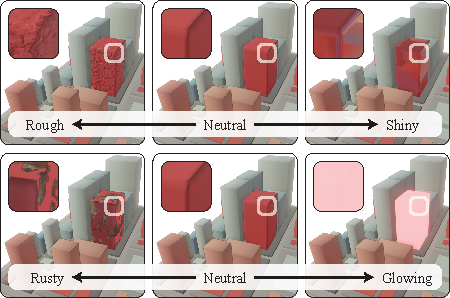
\includegraphics[width=1.0\linewidth]{item-based-metaphors}
	\caption{Two examples for item-based metaphors covering the transition between negative and positive object states.}
	\label{fig:item-based-metaphors}
\end{figure}

\subsection{Context-based Metaphors}
\noindent
\begin{figure*}[t]
	\centering
	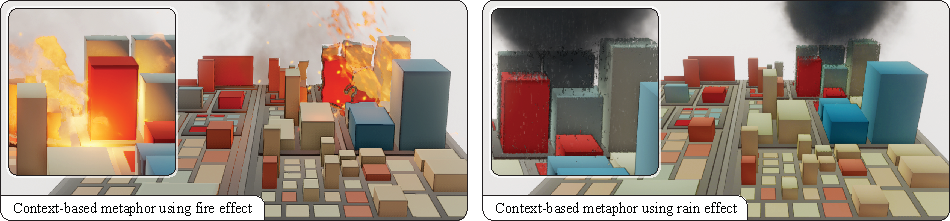
\includegraphics[width=1.0\textwidth]{context-based-metaphors}
	\caption{Context-based metaphors, automatically assigned to development hot spots (\eg strong decrease or stagnation).}
	\label{fig:context-based-metaphors}
\end{figure*}
Context-based metaphors are either natural phenomena or effects that affect the area surrounding treemap items or a group of adjacent items. 
In order to parametrize such effects properly, context-based metaphors require information about the hierarchical aggregation of software metrics to determine trends for parent items. 
Particle systems are mainly used to visually communicate hot spots (or regions-of-interest) in source code, \eg so-called \enquote{code smells}. 
Therefore, we use a fire effect or rain (\autoref{fig:context-based-metaphors}) to indicate negative trends.

\subsection{Trend-based Parametrization}
\noindent
To fully automate the trend-based parametrization, each effect contains a self description comprising all of its parameters. 
A single \emph{parameter description} consists of the \emph{parameter type} (\ie vector, scalar, and color), the value range $[i_{\mathrm{min}},\;i_{\mathrm{max}}]$ of the parameter $v$, a \emph{default value} and a boolean value that determines whether to \emph{inverse} the mapping or not (\eg a positive trend is mapped to a roughness of zero).
The parametrization is performed by mapping the trend $v$ from an input trend value range $[i_{\mathrm{min}},\; i_{\mathrm{max}}]$ to an output parameter value range $[j_{\mathrm{min}},\;j_{\mathrm{max}}]$ by 
$  v_{\mathrm{mapped}} = (v - i_{\mathrm{min}})\frac{j_{\mathrm{max}} - j_{\mathrm{min}}}{i_{\mathrm{max}} - i_{\mathrm{min}}} + j_{\mathrm{min}}$.
Every effect defines parameter sub-ranges that discretize the mapped parameter value $v_{\mathrm{mapped}}$ to the five categories: \emph{strong increase}, \emph{increase}, \emph{stagnation}, \emph{decrease}, or \emph{strong decrease}.

\subsection{Hierarchical Aggregation of Software Metrics}
\noindent
Similar to software maps, the hierarchical structure of trend map mirrors the directory tree of the current revision chosen from a code repository. 
To determine software metric trends for individual (\ie files) as well as groups of items (\eg packages), trend data is aggregated bottom-up within the hierarchy in a specified revision range.
Post-order and reversed level-order traversals are suitable for this task. 
Therefore, a node in a revision range tree holds a bucket $k$ for each revision within the revision range. 
The respective metric value  $x_k$ contained in the bucket is computed using \emph{weighted average}.
Empty buckets represent items that are not present in a specific revision. 
The weights $w_k$ are determined by counting the leaf nodes in the sub-tree where the node for which we want to aggregate the metric values is the root node.
